\section{Regression method based on SSPA database}
\label{se:correction_SI_method}
In order to improve the accuracy of the roll damping prediction, the SSPA database containing more than 250 roll decay tests with modern ships is used to propose new models. In the following preliminary investigation, two different approaches are used to build such a model for roll damping prediction. The model is assumed to be a function of the same input parameters as the SI-method (see equation \ref{eq:S1-method}). It was found in section \label{se:overall_comparison} that the $B_e$ coefficient changes a lot with the roll amplitude $\phi_a$. Three different options to approach this were considered:
\begin{itemize}
    \item Calculate $B_e$ for only one representative value of $\phi_a$
    \item Split into two regressions, one for $B_1$ and one for $B_2$.
    \item Calculate $B_e$ for a range of $\phi_a$ and include all in the regression
\end{itemize}
The first option was rejected because that would generate a model that works for one roll amplitude only, the second option was rejected because introducing two regression models was considered unnecessary complex. And it was also suspected that there could be correlations between $B_1$ and $B_2$ so that the two regressions needed to be connected in some way. So the third option was used which means that the $B_e$ used in the regression contains roll amplitudes between 0 and 10 degrees.  

\subsection{New regression model for roll damping}
The first approach further assume that the function can be expressed as a second order polynomial. Some statistical learning method is used to establish the regression model. The input parameters (the features) are first transformed into polynomial features including all possible coupling terms. The best polynomial features are selected using a feature selection algorithm, selecting the k best features \parencite[]{noauthor_sklearnfeature_selectionselectkbest_nodate} using a linear model for testing the individual effect of each of many regressors \parencite[]{noauthor_sklearnfeature_selectionf_regression_nodate}. Cross validation, as described in section \ref{se:cross_validation} below, is used to estimate the accuracy. The accuracy of using only the one best polynomial feature, only the two best polynomial features and so on is determined. In this way the optimum number of polynomial parameters is selected, as being the middle way between having enough features to describe the data but not over-fitting. A regression model with 12 polynomial features was found to have the best accuracy when evaluated in this way. The model was determined by fitting the selected regression model to the entire data, giving the following expression:

\begin{equation} \label{eq:polynom_complex}
\hat{B_{e}} = - 0.4743 A_{0} T + 0.002891 A_{0} V - 0.266 BK_{B} V + 0.007243 BK_{L} V - 0.02573 C_{b} V - 0.1077 OG V + 0.4026 T + 0.003985 V^{2} + 0.02227 V \hat{omega0} + 0.04347 V beam + 0.04084 V phi_{a} - 0.004035 V + 0.006761
\end{equation}

All the inputs with length scale ($T$, $B_{KB}, $B_{KL}$, $beam$) are nondimenilaized with $L_{pp}$. $V$ is nondimenionalized using $\sqrt{L_{pp}$. The middsection coefficients $A_0$ and block coefficients $C_b$ are already nondimensional. The roll amplitude $\phi_a$ is in radians.


\subsection{Correction based on Ikeda's method}
The second approach uses the SI-method as is, but then apply some corrections to the output damping components. A roll amplitude correction factor was also added. The correction factors have been determined by fitting a linear regression model to the roll damping components giving the following expression: 
\begin{equation} \label{eq:polynom_correction}
\hat{B_{e}} = 0.7396 \hat{B_{BK}} - 1.256 \hat{B_{E}} + 9.289 \hat{B_{F}} + 0.6891 \hat{B_{L}} + 0.6691 \hat{B_{W}} + 0.02178 phi_{a} - 0.003594
\end{equation}

The proposed correction factors implies that $\hat{B_{BK}}$ and $\hat{B_{W}}$ should be reduced, $\hat{B_{E}}$ should be made negative and $\hat{B_{L}}$ is not corrected much.

Work has been conducted to propose a correction to the SI-method based on the findings in this paper. The idea is to find correction factors that can be applied to the roll damping components calculated with the SI-method. In order to handle the problem of $\hat{B_e}$ accuracy being very much depending on the roll amplitude a roll amplitude correction factor has also added. The correction factors have been determined by fitting a linear regression model to the roll damping components, calculated with the SI-method at roll amplitudes between 0 and 10 degrees, giving the following expression: 
\begin{equation} \label{eq:polynom_correction}
\hat{B_{e}} = 0.7396 \hat{B_{BK}} - 1.256 \hat{B_{E}} + 9.289 \hat{B_{F}} + 0.6891 \hat{B_{L}} + 0.6691 \hat{B_{W}} + 0.02178 phi_{a} - 0.003594
\end{equation}

The proposed correction factors reduce $\hat{B_{BK}}$ and $\hat{B_{W}}$, removes $\hat{B_{E}}$ and $\hat{B_{L}}$ is not corrected much. 

\subsection{Cross validation}
When constructing a regression model from a data set, over-fitting the data can be a problem. Including too many parameters and/or allowing too high order of the model would give a very good representation of the present roll damping data, but large extrapolation errors when the model is used on other data. K-fold cross validation has been used to "mimic" this situation. The data has been split into five smaller sets (folds). Four of the folds are used to train the model and the fifth is used for testing (validation). The validation is done by calculating the coefficient of determination $R^2$ for the fitted model. This is done for all five possible train/test combinations. Applying the proposed correction improves the accuracy according to the cross validation results in table \ref{tab:crossvalidation} with an average $R^2$ of 0.68 compared to 0.47 without the correction. The improvement can also be seen when comparing figure \ref{fig:ikeda_components} with \ref{fig:ikeda_phi_a}.
\begin{tabular}{lrr}
\toprule
{} &  \$R\textasciicircum 2(SI-method)\$ &  \$R\textasciicircum 2(SI-corrected)\$ \\
\midrule
0 &              0.39 &                 0.66 \\
1 &              0.56 &                 0.71 \\
2 &              0.47 &                 0.66 \\
3 &              0.32 &                 0.69 \\
4 &              0.59 &                 0.66 \\
\bottomrule
\end{tabular}


\begin{figure}[H]
\vspace{-0.5cm}
\centering
  \centering
  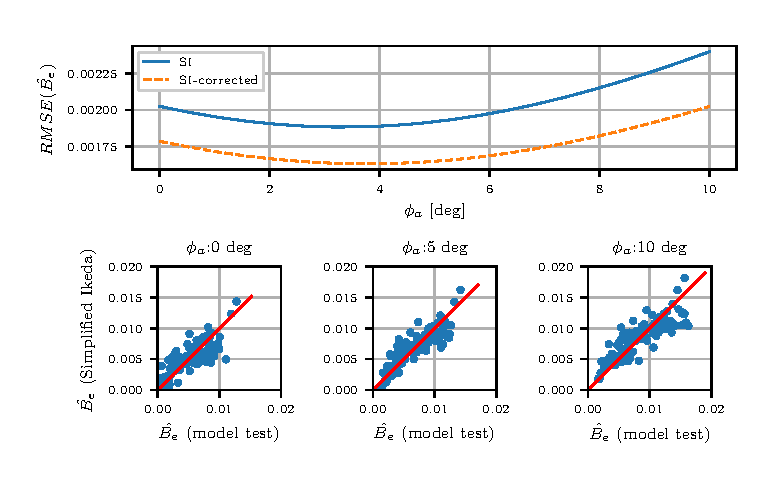
\includegraphics[]{figures/ikeda_corrected_phi_a.eps}
  \vspace{-0.5cm}
  \caption{Root mean square error of roll damping prediction between the SI-method, corrected SI-method and the model test results (upper plot). Influence of roll amplitude $\phi_a$ on $\hat{B_e}$ between the corrected SI-method and model tests for $0^{\circ}$ (bottom left plot), $5^{\circ}$ (bottom middle plot) and $10^{\circ}$ (bottom right plot), respectively.}
  \label{fig:ikeda_phi_a_correction}
\end{figure}
